%
\documentclass[12pt]{article}

%% make references and citations clickable
\usepackage[backref,colorlinks=true, linkcolor=blue, citecolor=blue, urlcolor=blue, pdfborder={0 0 0}]{hyperref}

%% set the paper geometry
\usepackage[left=1in,top=1in,right=1in,bottom=1in,letterpaper]{geometry}

%% this is for arrows with text over them  --- currently not installed
%%\usepackage{mathtools}

%% uncomment the next line if you need to present an algorithm
%\usepackage{algorithm,algorithmic}

% This section is added by me (Geoff)
%-----------------------------------------------
%% standard AMS stuff
\usepackage{amssymb,amsmath,amsthm}

%% some proof-writing environments
\newenvironment{claim}[1]{\par\noindent\underline{Claim:}\space#1}{}
\newenvironment{claimproof}[1]{\par\noindent\underline{Proof:}\space#1}{}
%\newenvironment{proof}{\paragraph{Proof:}}{\hfill}
\theoremstyle{definition}
\newtheorem{theorem}{Theorem}[section]
\newtheorem{ex}[theorem]{Example}
\newtheorem{defn}[theorem]{Definition}
\newtheorem{lemma}[theorem]{Lemma}
\newtheorem{notn}[theorem]{Notation}

%% norm and abs val and inner prod
\newcommand{\norm}[1]{\left\lVert#1\right\rVert}
\newcommand{\abs}[1]{\left\lvert#1\right\rvert}
\newcommand{\iprod}[1]{\langle #1 \rangle}
\newcommand{\spn}[0]{\text{span}}

%% ceiling and floor   --- Not working for some reason
%%\DeclarePairedDelimiter\ceil{\lceil}{\rceil}
%%\DeclarePairedDelimiter\floor{\lfloor}{\rfloor}

%% kernel and image  -- Currently did something wrong
%%\newcommand{\ker}[1]{\text{ker}\left(#1\right)}
%%\newcommand{\Im}[1]{\text{Im}\left(#1\right)}  %% TODO: FIX THIS

%% Important letters/symbols
\newcommand{\ep}[0]{\epsilon}
\newcommand{\R}[0]{\mathbb{R}}
\newcommand{\bR}[0]{\bar{\mathbb{R}}}
\newcommand{\cC}[0]{\mathcal{C}}
\newcommand{\cP}[0]{\mathcal{P}}
\newcommand{\pd}[0]{\partial}

%% I had some issues with alignment, here was one online soln
%%\usepackage[fleqn]{amsmath}
%% It DIDN'T WORK THOUGH

%------------------------------------------------


%% for including urls by \url{url text}
\usepackage{url}

\usepackage{graphicx}

\begin{document}

\title{Graph Laplacian Data Fusion applied to Optical/Lidar dataset}
\author{Geoffrey Iyer}
\maketitle

\section*{Preliminary Results}

I got the Nystrom Extension code to work with our example, and used it to calculate eigenvectors of the Graph Laplacian for a fusion of the Optical/Lidar data from the 2015 Data Fusion Contest.

Let $n = \left(\text{number of pixels}\right)$, and label them $\{x_1,\ldots,x_n\}$. Recall, for two pixels $x_i,x_j$, we define the weight
\[w_{ij} = \exp\left( - \max\left(\norm{x_i - x_j}_{\text{Optical}}, \norm{x_i - x_j}_{\text{Lidar}}\right)\right).\]
This gives us a weight matrix $W$, from which we construct the normalized Graph-Laplacian
\[L = I - D^{-\frac{1}{2}}WD^{-\frac{1}{2}}.\]
Here $D$ is the degree matrix, a diagonal matrix with
\[d_ii = \sum_{j=1}^n w_{ij}.\]
The eigenvectors of the graph laplacian correspond to solutions of the relaxed graph-min-cut problem.

For computational efficiency, we use the Nystrom Extension to avoid calculating the entire $W$. Instead we choose $m << n$, and calculate only $m$ columns of the full matrix $W$. This is enough to give us a reasonable approximation of the first $m$ eigenvectors of $L$ (where by 'first' I mean the eigenvectors corresponding to the smallest eigenvalues).

See the example pictures below. I've reprinted the original data, followed by the first 6 eigenvectors. The most important thing to notice here is that the eigenvectors are truly fusing the data. Compare the picture of the eigenvector\#1 to the lidar data, then to the optical data. You will see elements of both.

TODO list: \begin{itemize}
\item Lots of tuning of parameters
\item Use these eigenvectors to perform some sort of classification
\item Code can still be further optimized (currently it runs for these images in about 10 seconds, but there are operations that I know can be improved).
\end{itemize}

\begin{figure}
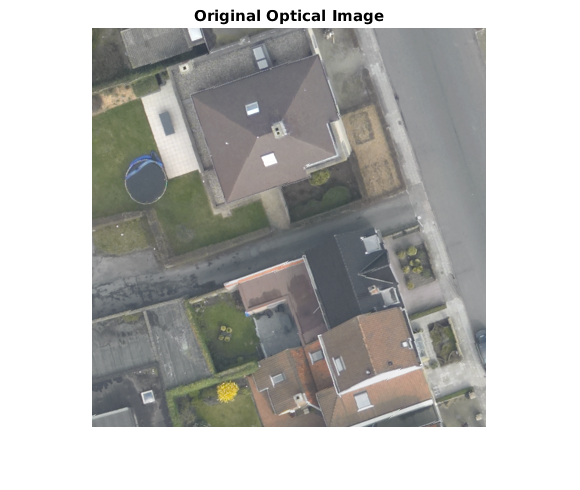
\includegraphics[width=\linewidth]{Optical.png}
\end{figure}

\begin{figure}
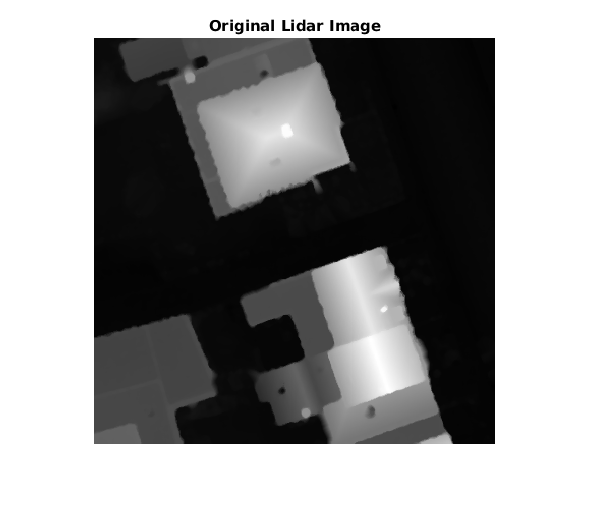
\includegraphics[width=\linewidth]{Lidar.png}
\end{figure}

\begin{figure}
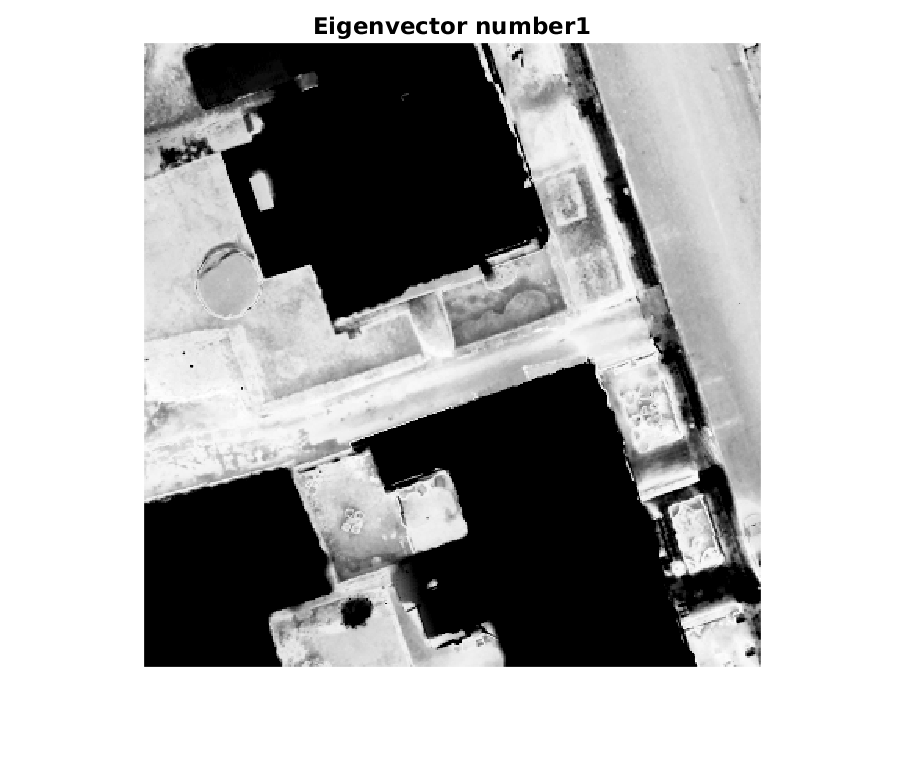
\includegraphics[width=\linewidth]{evec1.png}
\end{figure}

\begin{figure}
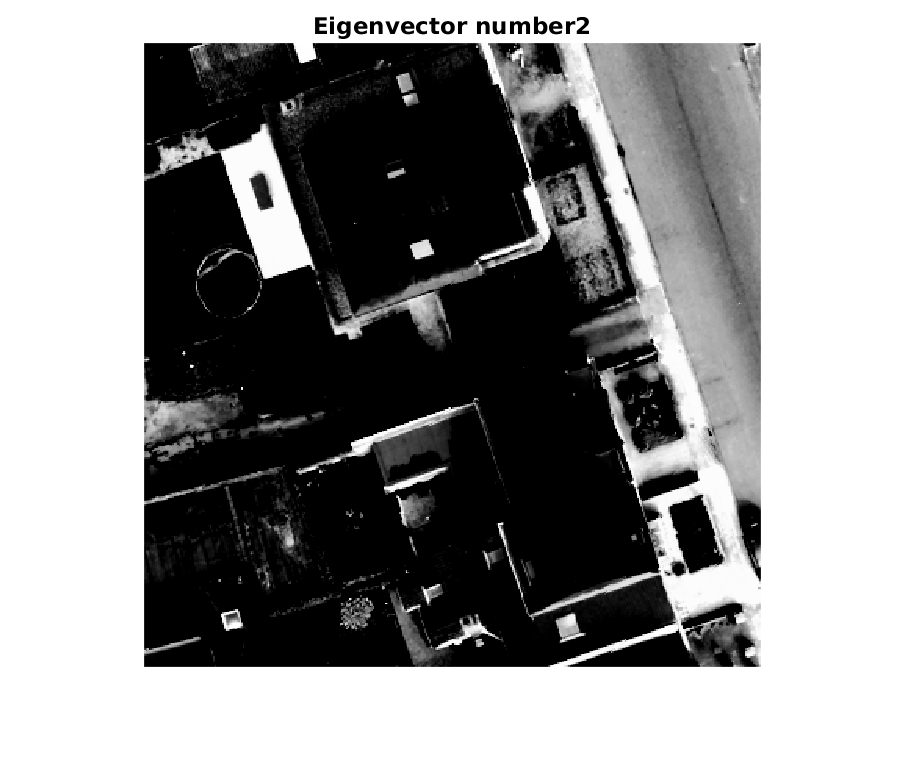
\includegraphics[width=\linewidth]{evec2.png}
\end{figure}

\begin{figure}
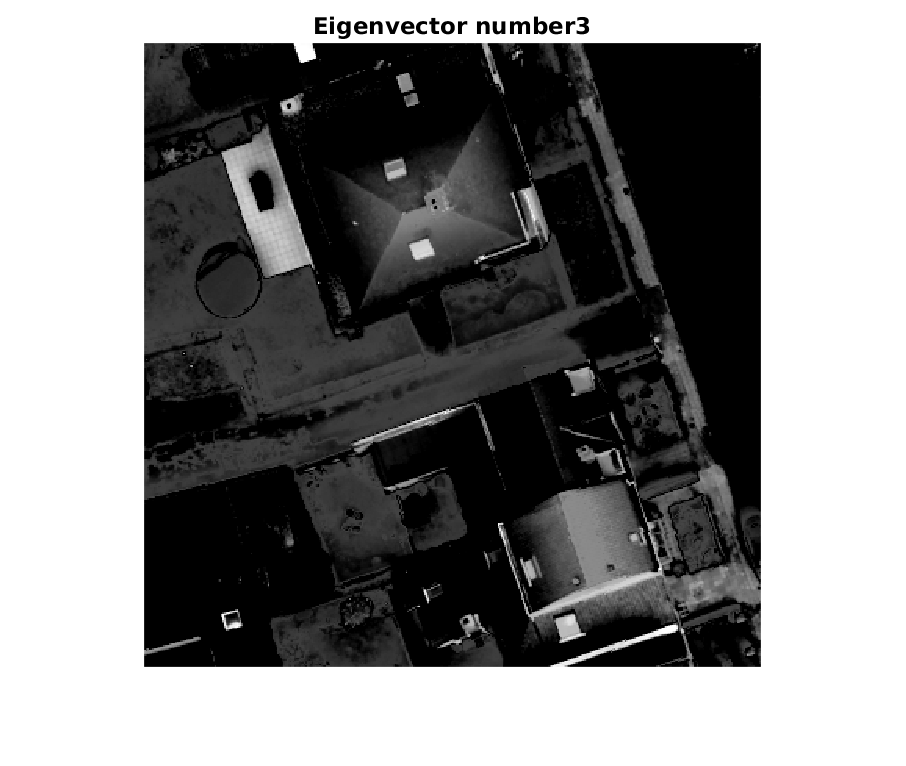
\includegraphics[width=\linewidth]{evec3.png}
\end{figure}

\begin{figure}
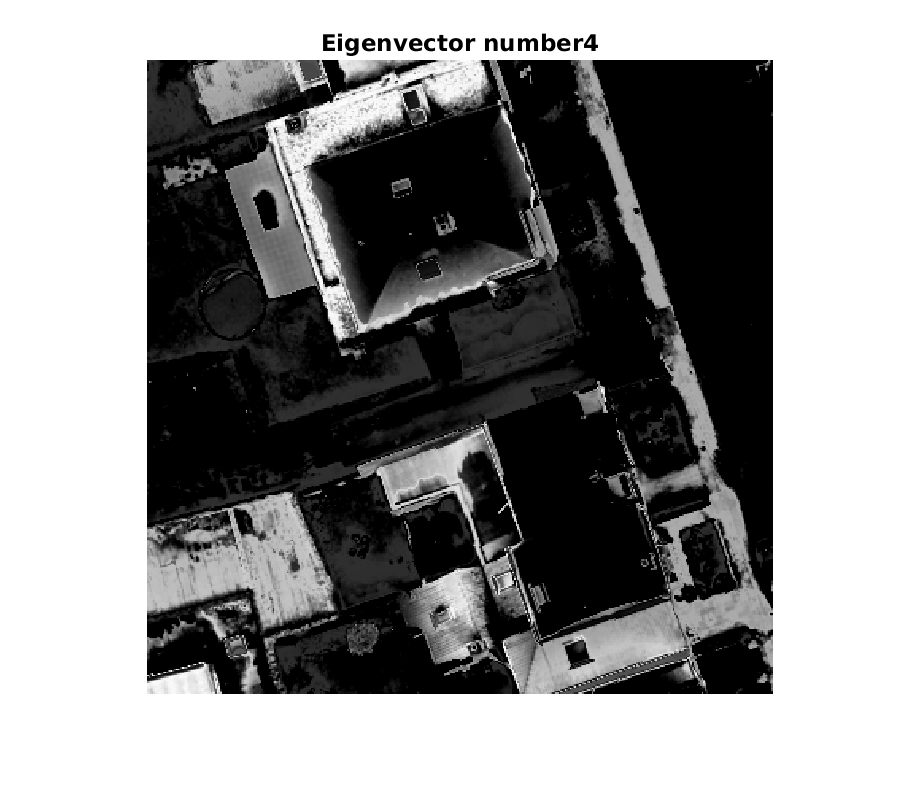
\includegraphics[width=\linewidth]{evec4.png}
\end{figure}

\begin{figure}
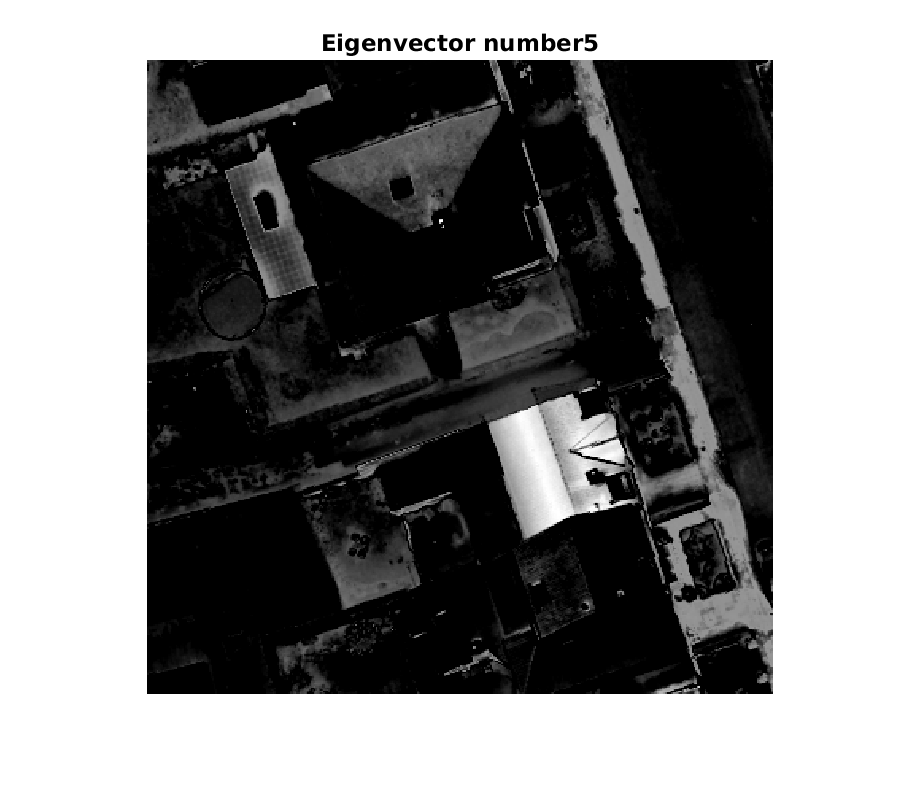
\includegraphics[width=\linewidth]{evec5.png}
\end{figure}

\begin{figure}
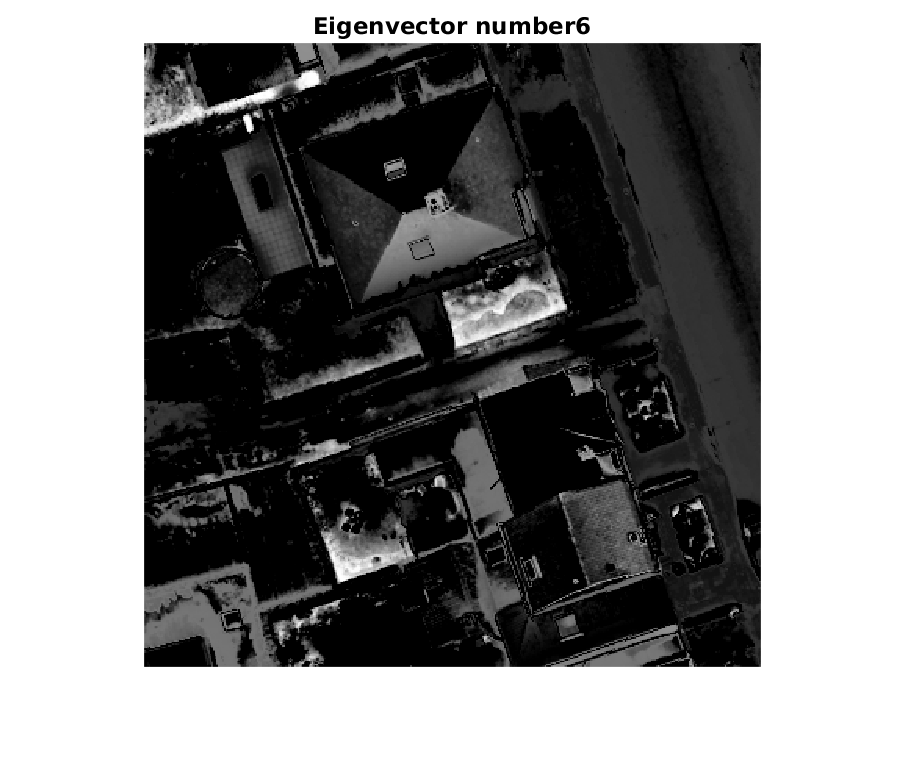
\includegraphics[width=\linewidth]{evec6.png}
\end{figure}

\end{document}
